\chapter{Diseño Termo-mecánico}

El presente capítulo tiene como propósito, utilizar la información y análisis recopilados a través de los capítulos anteriores para proponer una solución térmico-mecánica integral para el radio y la GRT, en consideración de todos los aspectos operativos actuales y deseados para la estación. Como su nombre lo indica la propuesta consta de dos parte fundamentales, la primera hace referencia a la solución térmica-pasiva propuesta, la cual se relaciona directamente con la parte mecánica, debido a la necesidad de adaptar un dispositivo electrónico a condiciones mecánicas y térmicas adversas a su diseño original.

\section{Contexto mecánico del radio}

Como ya antes se ha mencionado el radio es un dispositivo electrónico comercial  que se tiene que ajustar para otras condiciones como por ejemplo, su adaptación estructural dentro del gabinete. Para lo cual se debió realizar un modelo en 3D que permitiera el manejo del mismo dentro del espacio del gabinete.

\begin{figure}[H]
\centering
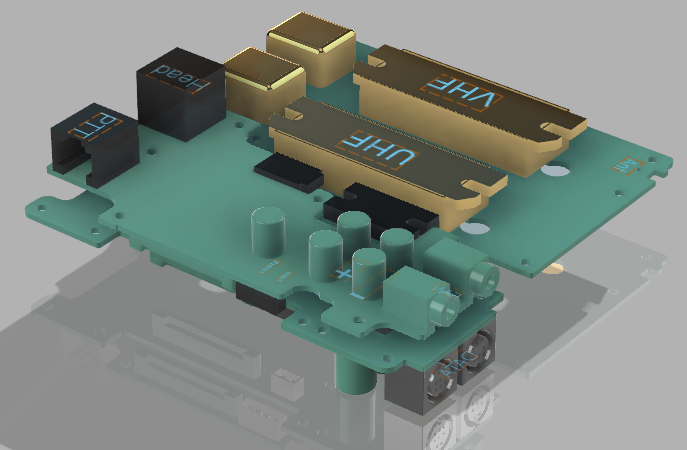
\includegraphics[scale=0.6]{Figuras/G5.png}
\caption{Render del Radio transmisor}
Fuente: Elaboración Propia
\label{G5}
\end{figure}

Una de las principales preocupaciones estructurales es asegurar el libre acceso a los módulos de potencia, sin comprometer la integridad del radio ni el acceso a los puertos que son requeridos para el manejo del radio durante las transmisiones. En la Figura \ref{G1} se muestra la disposición actual de los demás componentes de la estación diseñados hasta el momento. En los Anexos \ref{anexo16},\ref{anexo17},\ref{anexo18} y \ref{anexo19} se muestran imágenes reales del radio y su configuración física original. 

\begin{figure}[H]
\centering
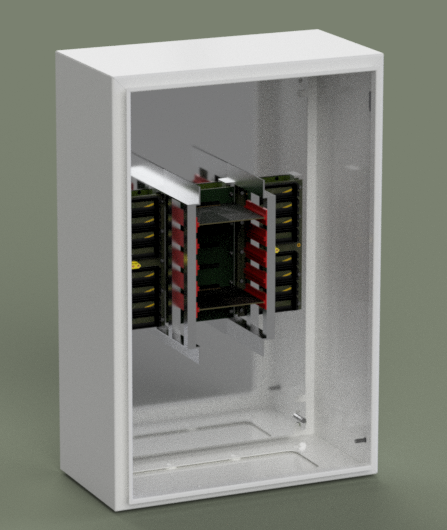
\includegraphics[scale=0.6]{Figuras/G1.png}
\caption{Render del estado actual de la GRT}
Fuente: Render de elaboración propia con datos del SETECLab
\label{G1}
\end{figure}

\begin{figure}[H]
\centering
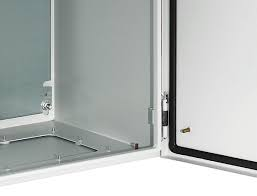
\includegraphics[scale=0.75]{Figuras/gabinete2.jpg}
\caption{Acceso inferior del gabinete}
Fuente: \cite{gabinete manual}
\label{acceso}
\end{figure}

Como se observa en las Figuras \ref{G1} y \ref{acceso} el gabinete cuenta con un acceso inferior para los cables, el mismo será el único utilizado tanto para el disipador como para el conector de la antena. Este último elemento es de vital importancia en la transmisión de los datos, lo que implica que la distancia entre el conector y el radio debe ser la mínima. Todas estas consideraciones convergen en la decisión de colocar el radio transmisor en la parte inferior del gabinete tal y como se muestra.

\begin{figure}[H]
\centering
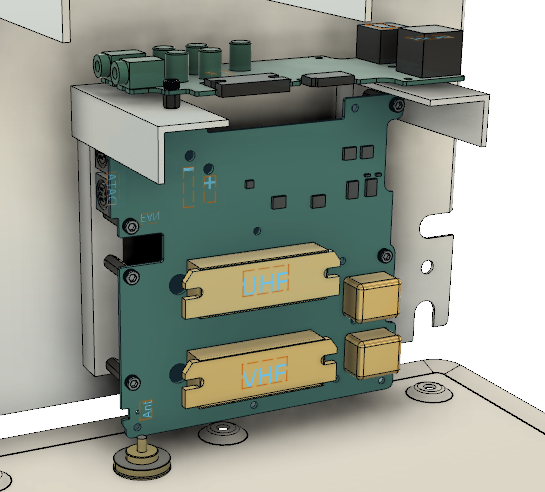
\includegraphics[scale=0.6]{Figuras/G3.png}
\caption{Montaje del radio}
Fuente: Elaboración Propia
\label{G3}
\end{figure}

\begin{figure}[H]
\centering
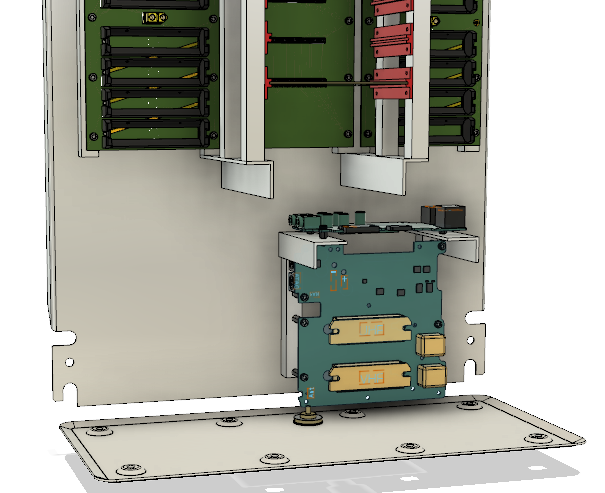
\includegraphics[scale=0.6]{Figuras/G4.png}
\caption{Vista General del Montaje}
Fuente: Elaboración Propia
\label{G4}
\end{figure}


En las Figuras \ref{G3} y \ref{G4} se logra apreciar como la placa secundaria (Figura \ref{secundaria}) se giro 90 grados con respecto a la placa principal (Figura \ref{principal}). Esto da solución al inconveniente de no poder separar las dos placas debido a los cables de comunicación que las unen entre sí y dan acceso libre a los módulos de potencia. Se debe recordar que el módulo en estudio es el marcado como $UHF$ en las distintas figuras.

\section{Propuesta de diseño}

Una vez conocida la posición del radio dentro del gabinete, se hace uso del recurso del modelo de la estación para plantear una solución térmica pasiva que mejore las condiciones operativas de la estación y del radio transmisor. En este punto del proyecto, la parte del modelo y la parte mecánica están estrechamente relacionadas, por lo que se echará mano a los recursos computacionales para optimizar los cálculos.

\subsection{Diseño de disipador}

Desde el punto de vista mecánico el disipador debe cumplir con las siguientes condiciones:

\begin{enumerate}
    \item No debe agregar fuerzas de tracción o de palanca sobre los módulos de potencia, los cuales están diseñados para una disposición horizontal no vertical.
    \item El disipador debe ser capaz de aprovechar las corrientes de aire desde cualquier dirección, ya que, como se observó en los datos meteorológicos la dirección del viento es muy variable y no se puede garantizar aún la posición del GRT sobre la torre, de manera que se desconoce si dicha ubicación concuerda con la dirección de las ráfagas de mayor intensidad.
    \item El disipador en general debe ser de fácil montaje, desmontaje, y construcción, de manera que pueda ser construido y ensamblado por los mismos estudiantes o integrantes del laboratorio 
\end{enumerate}

\textbf{Estimación del área mínima de transferencia para el disipador:} Utilizando la Ecuación \ref{Newton} de la ley de enfriamiento de Newton, se puede realizar una estimación del área superficial de transferencia con la suposición válida de que el coeficiente de convección es constante durante el proceso y que la temperatura en la superficie de las aletas del disipador es regular en toda la superficie. \cite{cengel}

Durante los experimentos se observó que el flujo del calor del radio hacia el medio no superaba los \SI{0,3}{\watt}, por lo que la estimación del área mínima de convección se estimará con un flujo de calor de \SI{0,5}{\watt} a manera de factor de seguridad. Por lo tanto

\begin{equation}\label{area minima}
    A=\frac{Q}{h(T_{s}-T_{\infty })}\;\;(\si{\watt})
\end{equation}

Donde los valores utilizados para las variables son:

\begin{table}[H]
\centering
\caption{Estimación del área mínima}
\label{calculo20}
\begin{tabular}{cccc}
\toprule
\textbf{Variable} & \textbf{Valor}  & \textbf{Unidad}      & \textbf{Ecuación utilizada} \\ \midrule
$Q$ & 0,5  & \si{\watt} & Parámetro de diseño \\
$h$ & 14,57 & \si{\watt/\square\meter\celsius} & Parámetro de diseño
\\
$T_{s}$ & 40 & \si{\celsius}& Parámetro de diseño\\
$T\infty$ & 30,45 & \si{\celsius} & Parámetro ambiental\\
\bottomrule
\end{tabular}
\end{table}

Se obtiene un área mínima de:

\begin{equation}\label{resultado area}
    A_{min}= 3,59\times 10^{-3}\;(\si{\square\meter})
\end{equation}

El resultado obtenido parte de la suposición de que el disipador estará a la temperatura superficial mostrada como parámetro de diseño de punto de operación para el módulo, por ende una área menor a la calculada implica una temperatura igual o mayor a las que el radio alcanza actualmente. Si utilizáramos el área mínima obtenida y lo extendiéramos en una superficie cuadrada, se obtendría un cuadrado de aproximadamente $6X6$ \si{\centi\meter}, lo cual es relativamente pequeño.

\textbf{Propuesta de Disipador:} Considerando la manufactura del disipador se optará por una geometría cilíndrica vertical, a diferencia de las configuraciones rectangulares tradicionales; esto debido a que desde el punto de vista de manufactura, una barra cilíndrica es más fácil de maquinar que una rectangular; por otro lado desde el punto de vista de transferencia de calor, esta geometría permite aprovechar las ráfagas de viento provenientes de cualquier dirección independientemente de la orientación de la estación en la torre.

\begin{figure}[H]
\centering
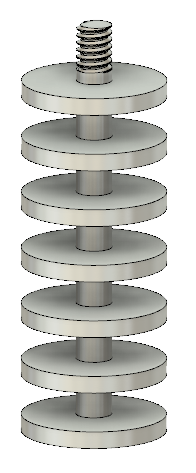
\includegraphics[scale=0.6]{Figuras/heat_sink.png}
\caption{Propuesta de disipador}
Fuente: Elaboración Propia
\label{heat_sink}
\end{figure}

Por facilidades constructivas para el diseño se propone utilizar una barra de aluminio de $1\,in$ (\SI{25,40}{\milli\meter}) y realizar reducciones con un torno convencional a diámetros internos de $1/4\,in$ (\SI{6,35}{\milli\meter}), dándole así forma a las aletas de (\SI{3}{\milli\meter}) de espesor. El espaciado entre las mismas se determina según lo analizado en el marco teórico

\begin{table}[H]
\centering
\caption{Distanciamiento Óptimo para las aletas}
\label{resultado_sopt}
\begin{tabular}{cccc}
\toprule
\textbf{Variable} & \textbf{Valor} & \textbf{Unidad} & \textbf{Ecuación utilizada} \\ \midrule
$Ra_{L}$ & \num{1,3176e4} & $N/A$ & \ref{ra1}           \\
$L$  & 0,0254               & \si{\meter}   & Parámetro de diseño \\
$S_{opt}$   & 0,0068  & \si{\meter} & \ref{sopt}    \\
$n$ & 7 & $N/A$ & \ref{numeroaletas}        \\ \bottomrule
\end{tabular}
\end{table}

Al realizar el diseño mostrado en la Figura \ref{heat_sink} se obtuvo finalmente una área superficial real de \num{6,57e-3}\si{\square\meter}, lo cual es \num{1,83} veces más que el área mínima; sin embargo como se observó en el modelo de la estación, la radiación solar tiene un impacto significativo en la temperatura interna del gabinete por lo que para efectos del proyecto se utilizarán dos de estos disipadores, con el fin minimizar este impacto de la estación sobre el radio.

Considerando todos estos aspectos, la ubicación del radio en la estación y la geometría y ubicación de los módulos de potencia se realiza la siguiente propuesta de disipador.

\begin{figure}[H]
\centering
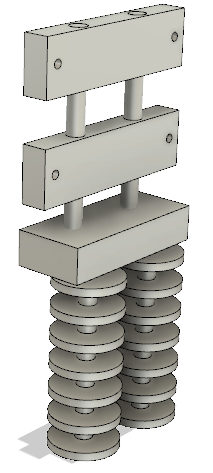
\includegraphics[scale=0.6]{Figuras/heat_sink_completo.png}
\caption{Propuesta completa de disipador}
Fuente: Elaboración Propia
\label{heat_sink_completo}
\end{figure}

Con la propuesta mostrada en la Figura \ref{heat_sink_completo} se pretende abarcar los dos módulos de potencia mediante las placas horizontales, darle un camino al flujo de calor mediante las dos barras que las atraviesa, y llegar a una base que sirve de soporte dentro del gabinete, pero a la vez de conexión con el exterior y los disipadores. Más adelante se detalla su interfaz con el radio transmisor y con el gabinete. Por otro lado los planos constructivos se encuentran en los anexos

\section{Modelo térmico del disipador:}

El esquema de modelado para esta ocasión, consiste en partir del modelo para la estación y agregarle los bloques y parámetros que simulen el comportamiento térmico del disipador y determinar el impacto que el mismo tendría en el radio y la estación.

\textbf{Pasta térmica:} Para efectos de cálculos, por lo general cuando se trata de transferencia de calor por conducción , se asume que las superficies en contacto son lisas, lo cual en la realidad no es cierto; la rugosidad del material genera un efecto conocido como resistencia de contacto, y esta asociada a las pequeñas burbujas de aire que se forma entre las rugosidades de ambos materiales. Este efecto no suele ser despreciable para situaciones como esta sin embargo, su determinación suele ser experimental y complicada de realizar. \cite{cengel}

Los módulos de potencia por su parte poseen superficies pulidas con el fin de reducir este efecto y como sucede en la mayoría de estos casos se hace uso de una pasta térmica, la cual genera una capa uniforme conductora de calor, que elimina estas pequeñas burbujas y crea una interfaz entre las rugosidades de ambos materiales. La pasta térmica a utilizar posee un coeficiente de conductividad térmica de: \cite{pasta}

\begin{equation}\label{kpasta}
    k_{pasta}=1,172\;\;(\si{\watt/\meter\cdot\kelvin})
\end{equation}

\textbf{Barras conductoras:} Como se muestra en la Figura \ref{heat_sink_completo} las barras representan un medio de transferencia entre la interfaz módulo-placa y la interfaz base-disipador por lo que se debe considerar la conducción térmica a través de las mismas, para lo cual se utilizan las propiedades para el Aluminio 60661-T6; el diámetro de estas barras es de$1/4\,in$ (\SI{6,35}{\milli\meter}).

\begin{table}[H]
\centering
\caption{Parámetros para la conductividad de las barras}
\label{barras}
\begin{tabular}{cccc}
\toprule
\textbf{Variable} & \textbf{Valor}          & \textbf{Unidad} & \textbf{Ecuación utilizada} \\ \midrule
$k_{Al}$& 167 & \si{\watt/\meter\cdot\kelvin} &\cite{aluminio}      \\
$A_{total}$ & \num{2,53355e-4} & \si{\square\meter} & Parámetro de diseño   \\ \bottomrule
\end{tabular}
\end{table}

Para efectos del modelo la parte de convección externa, se utilizará el mismo bloque empleado en el modelo de la estación con la corrección respectiva en el área superficial de transferencia.

\subsection{Resultados del modelo térmico}

A partir de la experiencia del modelo de la estación, se propuso realizar dos casos de simulación, en donde se varié la radiación para observar su impacto tanto en el radio como en la estación. En el primer caso se utiliza el valor de radiación usado para el modelo de la GRT (caso \SI{100}{\percent} radiación); y un segundo caso en donde se reduce la radiación en un \SI{50}{\percent} de la utilizada.

\textbf{Caso 1}

\begin{figure}[H]
\centering
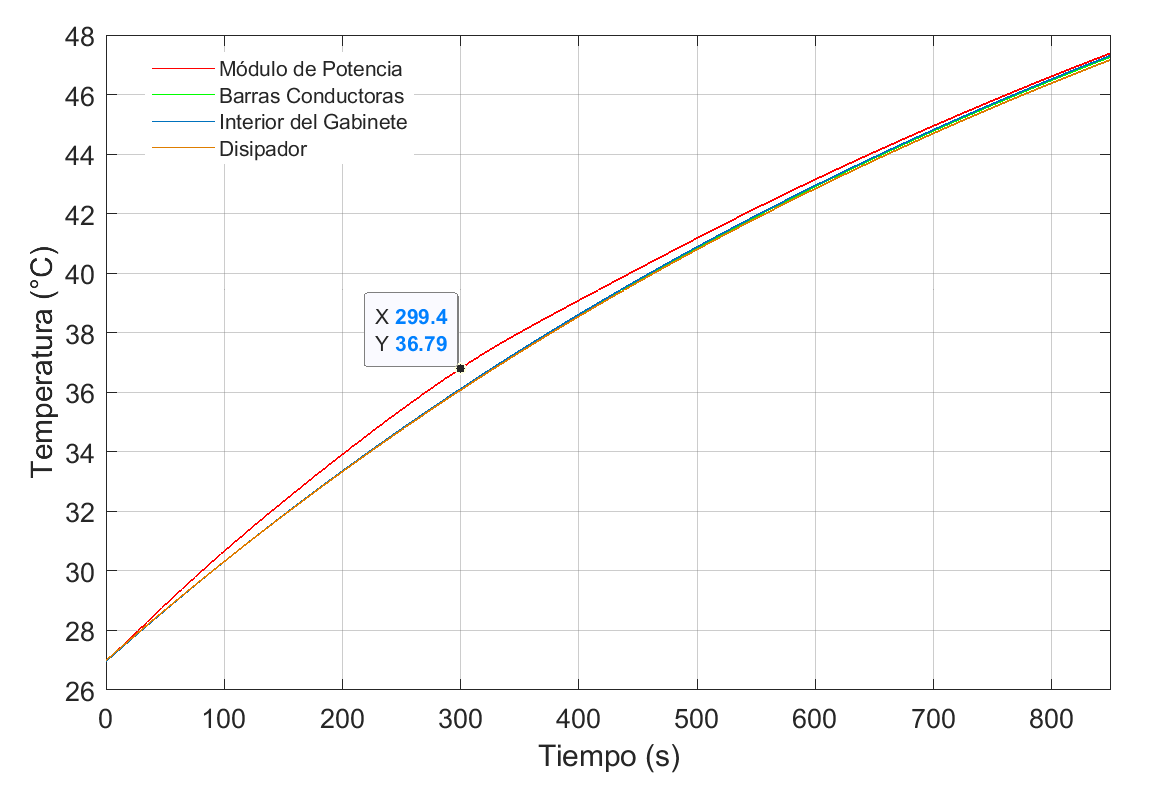
\includegraphics[scale=0.65]{Figuras/disipador_T.eps}
\caption{Gráfico temperatura vs tiempo para el modelo del disipador}
Fuente: Elaboración Propia
\label{disipador T}
\end{figure}

\begin{figure}[H]
\centering
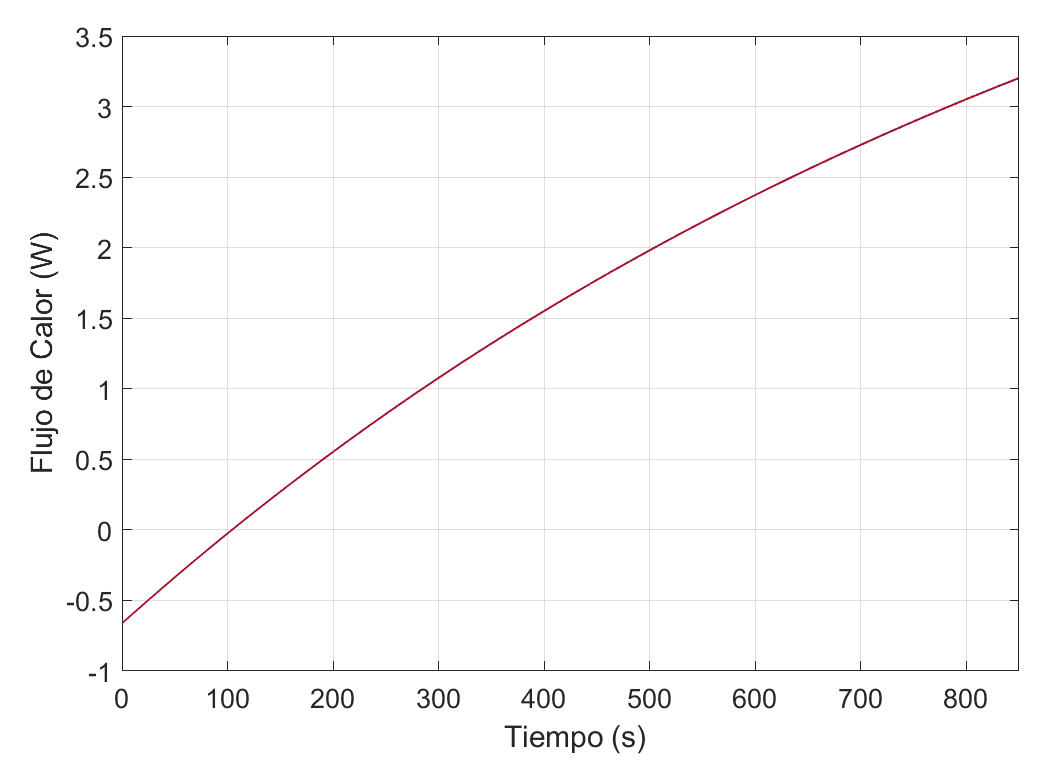
\includegraphics[scale=0.75]{Figuras/disipador_Q.eps}
\caption{Gráfico Flujo de calor vs tiempo del disipador}
Fuente: Elaboración Propia
\label{disipador Q}
\end{figure}

\begin{figure}[H]
\centering
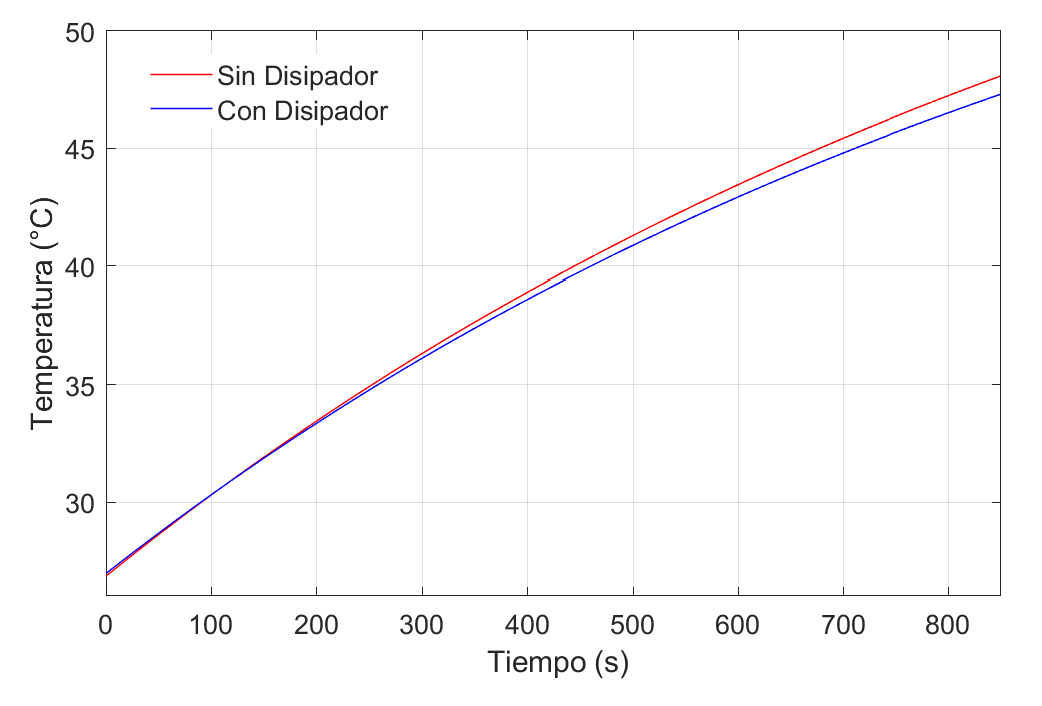
\includegraphics[scale=0.75]{Figuras/disipador_comparacion.eps}
\caption{Gráfico comparativo de la temperatura interna del gabinete}
Fuente: Elaboración Propia
\label{disipador comparacion}
\end{figure}

\textbf{Caso 2}

\begin{figure}[H]
\centering
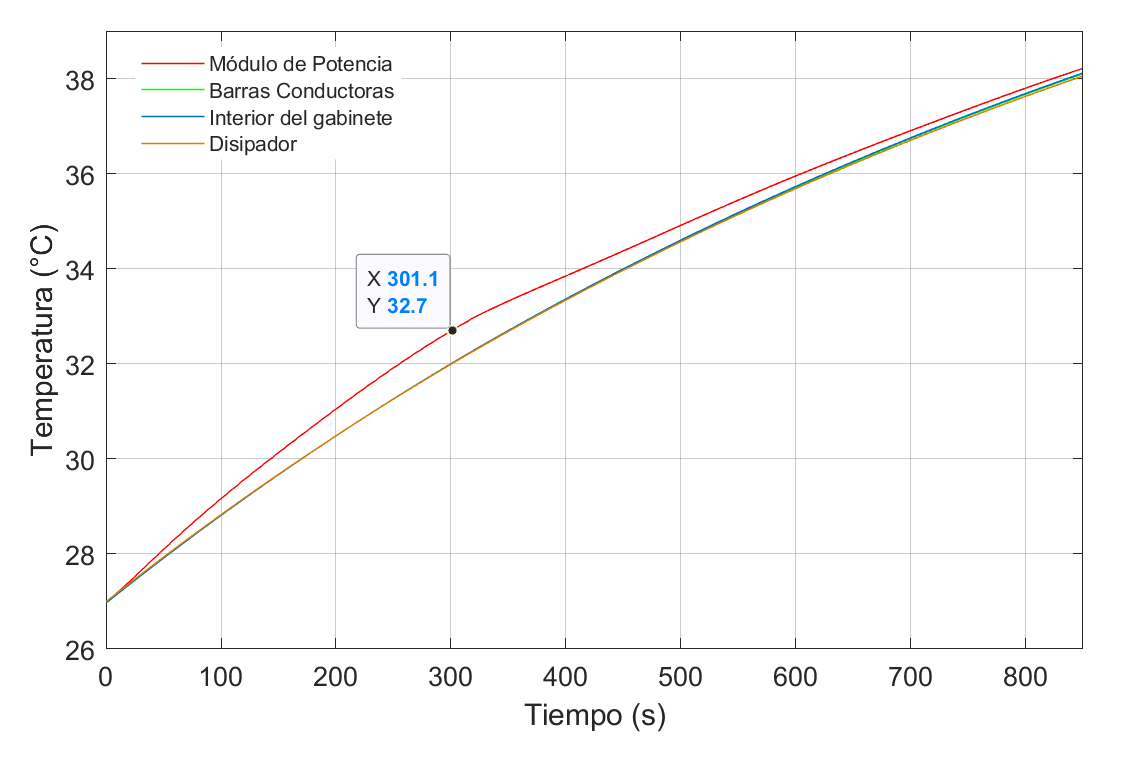
\includegraphics[scale=0.68]{Figuras/disipador_T_2.eps}
\caption{Gráfico temperatura vs tiempo para el modelo del disipado para el segundo caso}
Fuente: Elaboración Propia
\label{disipador T2}
\end{figure}

\begin{figure}[H]
\centering
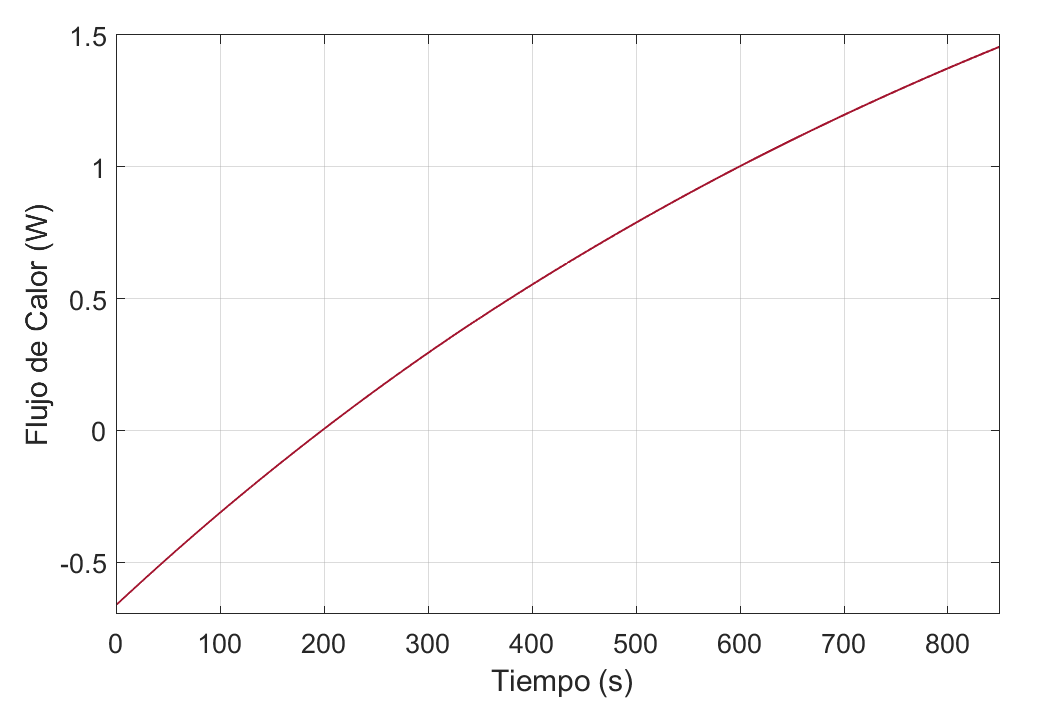
\includegraphics[scale=0.69]{Figuras/disipador_Q_2.eps}
\caption{Gráfico Flujo de calor vs tiempo del disipador para el segundo caso}
Fuente: Elaboración Propia
\label{disipador Q2}
\end{figure}

\begin{figure}[H]
\centering
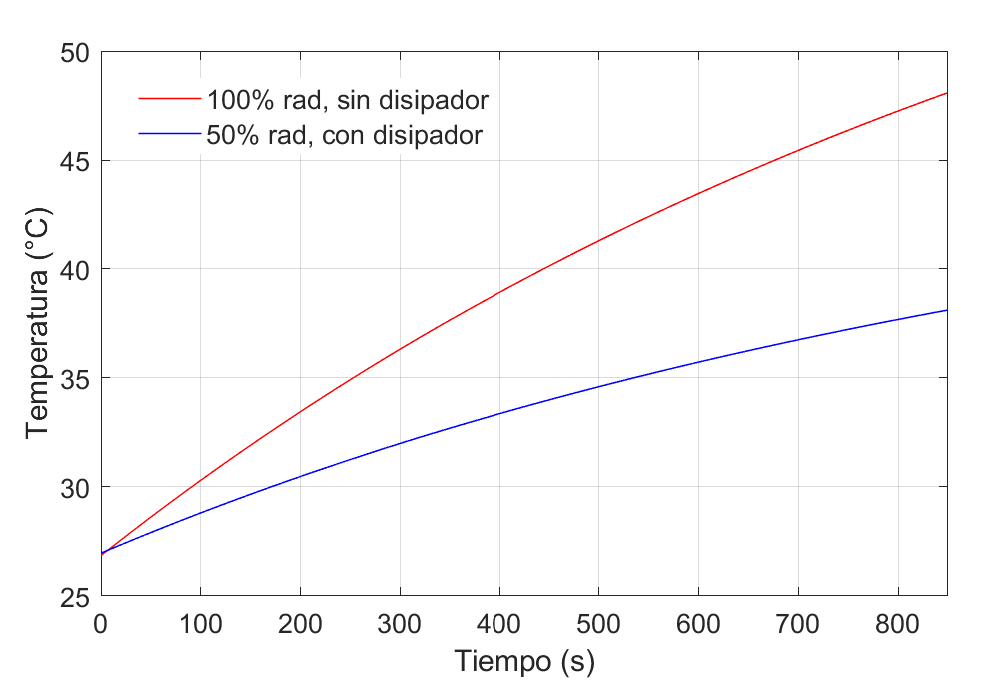
\includegraphics[scale=0.75]{Figuras/disipador_comparacion_2.eps}
\caption{Gráfico comparativo de la temperatura interna del gabinete para el segundo caso}
Fuente: Elaboración Propia
\label{disipador comparacion2}
\end{figure}

\subsection{Análisis del Resultado}

De la propuesta de diseño y de las simulaciones presentadas se pueden extraer las siguientes observaciones:

\begin{enumerate}
    \item Si se analiza el comportamiento del módulo de potencia, en cualquiera de los dos casos el disipador representa una mejoría notable en el comportamiento térmico del radio.
    \item En la Figura \ref{disipador comparacion} se observa como el gabinete presenta una leve mejoría debido al disipador, aún cuando este no esta dimensionado en función del manejo de la radiación.
    \item Cuando se compara el primer caso con el segundo, se ratifica la relevancia que tiene la radiación en el comportamiento térmico de la estación, y esto se observa claramente en la Figura \ref{disipador comparacion2} donde al reducir la radiación en un \SI{50}{\percent}, la temperatura tanto de gabinete como del radio se reduce significativamente.
    \item Basado en la observación anterior, se plantea la necesidad de una solución de carácter externo a la estación que reduzca el impacto o el porcentaje de radiación que llega al gabinete, como por ejemplo una estructura que genere sombra sobre el gabinete.
    \item En los dos casos se logra mantener el módulo de potencia dentro del rango operativo del mismo, de igual manera sucede con el punto de operación del radio en general. A pesar de que se observe  una tendencia a la alza en tiempo donde es difícil determinar su punto de estabilización, se debe recordar que desde el punto de vista real, los valores de radiación no se mantienen constantes, estos están en continuo aumento y disminución con respecto al promedio y varían significativamente entre periodos de \SI{15}{\min} según los datos de la estación de la OTS.
    \item A pesar de que el disipador amortigua el calentamiento del radio, una vez finalizada la transmisión se observa como debido a la radiación, el módulo sigue aumentando la temperatura en concordancia con los demás elementos y en dirección del equilibrio térmico.
    \item En cuanto a los flujos de calor, en ambos casos se superan los valores necesarios estimados para el módulo, y por el contrario se observa que dentro de la capacidad de los disipadores, estos asumen progresivamente la carga térmica del aire interno del gabinete.
    \item El valor negativo en los flujos de calor indica, para el inicio de la simulación según las condiciones internas del gabinete, que existe un diferencial de temperatura inverso a la dirección deseada del calor, tal y como se observa en las Figuras \ref{disipador comparacion} y \ref{disipador comparacion2}; conforme se da el aumento de temperatura el flujo de calor se invierte en la dirección deseada de adentro hacia afuera. Esto marca una de las implicaciones del disipador, ya que en momentos donde la temperatura ambiente sea mayor a la interior el flujo de calor se invertirá, por lo que el disipador siempre funcionará como un estabilizador térmico.
\end{enumerate}

\section{Validación del Diseño}

Para la validación tanto del diseño como del modelo para el disipador, se hizo uso de la herramienta de simulación de $Fusion 360$, la cual a parte de una validación, permite tener una mejor aproximación del comportamiento térmico del disipador y de cada uno de sus elementos que por una u otra razón no pudieron ser incluidos dentro del modelo. El software utiliza la resolución por medio de diferencias finitas, esto implica que se debe definir un tamaño de malla, entre más fina sea la malla, se aprecian mejor los cambios a través de los elementos. Para este caso se específicá un tamaño de malla de \SI{1}{\milli\meter}.

La simulación contempla al radio como una rampa de calor interno asociado a una temperatura en la placa superior, en el caso de las barras se considera un calor interno constante a manera de conducción al igual que para la base y finalmente en los disipadores se aplicó las condiciones de calor interno, convección y radiación desde el disipador hacia el exterior. Para la rampa de calor interno el parámetro inicial es una temperatura ambiente de \SI{30,45}{\celsius} a \SI{0}{\watt} con una condición final de \SI{75}{\celsius} a \SI{0,2}{\watt}, lo cual representa aproximadamente el comportamiento del radio en el modelo de la estación.

Debido a características propias del modelo donde solo se incluye el disipador y a la dificultad de agregar los demás elementos de la estación, esta simulación no se incluye la radiación solar ni la relación del disipador con respecto al gabinete.

\begin{figure}[H]
\centering
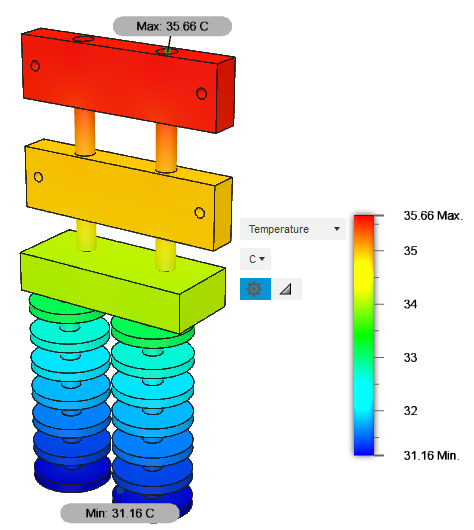
\includegraphics[scale=0.71]{Figuras/simulacion_1.png}
\caption{Resultados de la simulación en Fusión 360}
Fuente: Elaboración Propia
\label{simulacion1}
\end{figure}

Los puntos marcados en las Figuras \ref{disipador T} y \ref{disipador T2}, se colocaron para poder realizar la comparación con la Figura \ref{simulacion1}, ya en ese punto es donde la transmisión del radio finaliza y se obtiene la máxima temperatura posible entregada por el flujo del calor proveniente del módulo de potencia, en este punto se observa que tanto para el modelo como para la simulación las temperaturas son próximas entre sí, tanto para la placa del módulo como para el disipador, en este caso la simulación presenta la ventaja de que contempla una distribución real de las temperaturas sobre el área de transferencia para el disipador. Por otra parte se logra apreciar de igual manera el impacto que tienen los demás elementos como la base y la placa del segundo módulo, factores que no pudieron ser contemplados en el modelo sin embargo, esta simulación demuestra que dicho modelo es una buena aproximación de las condiciones del disipador dentro del gabinete.

\section{Solución termo-mecánica}

\subsection{Montaje final}

Uniendo la propuesta de ubicación de radio, a la propuesta de diseño del disipador, se obtiene como resultando el montaje mostrado a continuación. 
\begin{figure}[H]
\centering
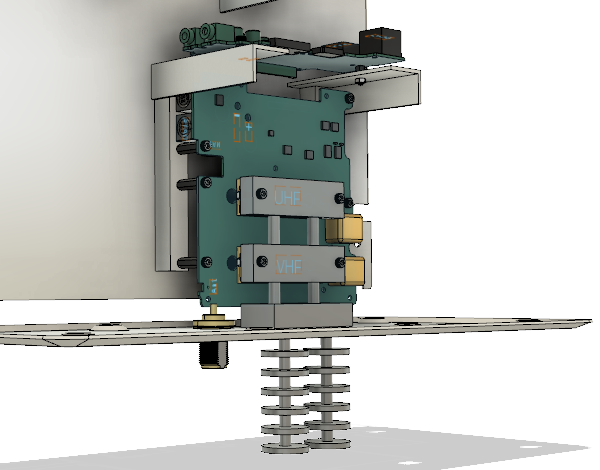
\includegraphics[scale=0.65]{Figuras/G7.png}
\caption{Vista General del montaje}
Fuente: Elaboración Propia
\label{solucion1}
\end{figure}

En la Figura \ref{solucion1} se observa como las placas de aluminio se adaptan a los dos módulos de potencia mediante tornillos de sujeción en conjunto con tuercas hexagonales por la parte posterior del radio. Por otra parte también se observa como los dos disipadores quedan por la parte externa, los mismos funcionan como medio de sujeción entre la placa base y la platina de acceso del gabinete por medio de las partes roscadas de ambos elementos. Esto presenta la ventaja de que se requieren solamente dos agujeros sobre la placa de acceso para la instalación de los disipadores y la sujeción de la base de las barras conductores, sin la necesidad de agujeros extra para una sujeción aparte de la base.

\begin{figure}[H]
\centering
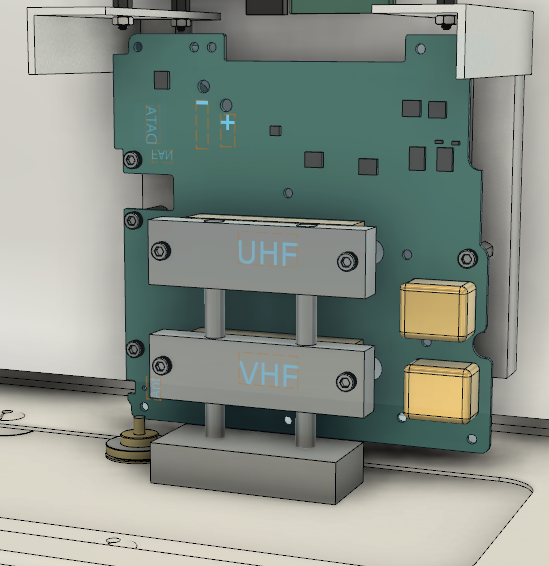
\includegraphics[scale=0.45]{Figuras/G11.png}
\caption{Vista interna del montaje}
Fuente: Elaboración Propia
\label{solucion2}
\end{figure}

Una de las principales consideraciones en el diseño era no agregar esfuerzos mecánicos adicionales a los módulos de potencia, por lo que se decidió que los mismos solamente irían sujetos a las placas de aluminio, las cuales son atravesadas por las barras conductoras sin embargo, las mismas no están sujetas mecánicamente a las placas, tal y como se observa en la Figura \ref{solucion3}. Las barras conductoras van roscadas sobre la base, la cual va fijada en su posición por los disipadores que funcionan a manera de contra rosca como ya antes se mencionó.\\

\begin{figure}[H]
\centering
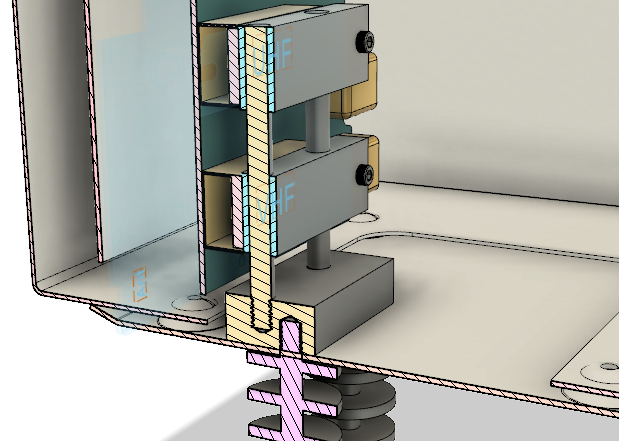
\includegraphics[scale=0.5]{Figuras/G12.png}
\caption{Vista de Sección}
Fuente: Elaboración Propia
\label{solucion3}
\end{figure}  %JR: que chuzo se ve

Por otra parte en la Figura \ref{solucion4} se observa la disposición del radio con respecto al gabinete, y es apreciable como el radio se encuentra ligeramente ubicado del centro hacia la derecha del gabinete, esto con el propósito e intención de dejar espacio suficiente para el panel frontal del radio el cual no puede encontrarse desconectado del radio; el mismo no se contempla dentro de la solución mecánica ya que aún no se ha definido su disposición final dentro de la estación, además el mismo no será retirado de su carcasa de fábrica por lo que cuenta con elementos de sujeción que le permiten ser adaptado o colocado dentro del gabinete con facilidad.

\begin{figure}[H]
\centering
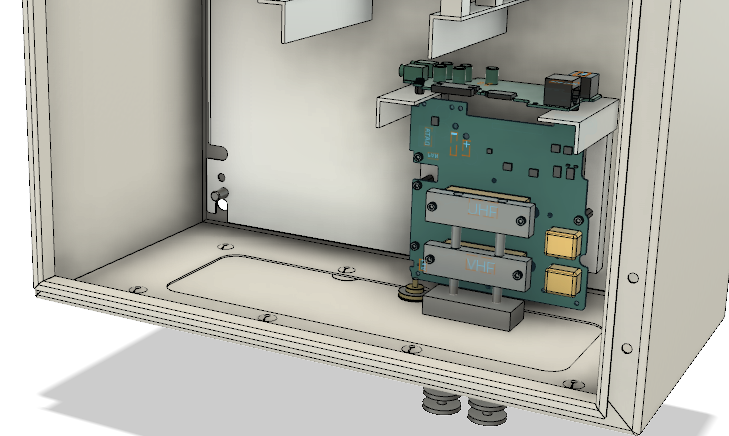
\includegraphics[scale=0.5]{Figuras/G9.png}
\caption{Disposición interna en el gabinete}
Fuente: Elaboración Propia
\label{solucion4}
\end{figure}

El procedimiento de instalación es sencillo, consiste en primero colocar la base por la parte interior del gabinete y enroscar desde la parte exterior los disipadores, una vez se encuentre fija la base se procede a enroscar las barras conductoras sobre la base para finalmente introducir las placas de los módulos en las barras conductoras y ajustar la altura a la de los módulos respectivos de manera que puedan ser fijados contra los módulos.

Una ventaja extra de este diseño, es la posibilidad de agregar más disipadores en la base con simples modificaciones, o bien al mantener la rosca original se puede aumentar el número de aletas en caso de ser necesario, lo que le da adaptabilidad al diseño. Además, en ambientes salinos, existe la posibilidad de corrosión en el aluminio, por lo que esta configuración mecánica permite su fácil reemplazo.

Dentro del montaje mecánico del radio, se veló por el acceso libre a los puertos que serán utilizados durante la misión, cabe aclarar que no son todos los puertos disponibles en el radio, lo cual permitió su orientación propuesta. Finalmente en los anexos se muestran los planos constructivos para el caso del disipador, así como otras figuras que evidencian disposiciones del radio dentro del gabinete.

\subsection{Humedad dentro del gabinete}

La solución térmica pasiva propuesta, resuelve el problema de carga térmica sensible del radio, mas no es una respuesta óptima para la carga térmica latente que representa la humedad sin embargo, para los gabinetes que poseen sistemas de refrigeración mecánico, una de las principales recomendaciones de los fabricantes como Hoffman es trabajar en puntos de operación más elevados de lo habitual, para garantizar que la temperatura de las superficies internas estén siempre por encima de la temperatura de rocío. En el caso de la GRT la misma ya cumple con estas condiciones de operar durante el día a temperaturas internas por encima de la temperatura ambiente, lo que deja a las horas de la tarde y nocturnas, así como cambios súbitos de clima, la posibilidad de que provoquen condensación. \cite{risoul}

Sin embargo, esto es posible solamente si existe un flujo libre de aire húmedo externo que ingrese en el gabinete, o bien algún sistema de refrigeración o ventilación que inyecte esta humedad dentro del mismo, por lo que la solución a la humedad para la GRT se reduce a dos acciones clave:

\begin{enumerate}
    \item Eliminar las infiltraciones de aire húmedo debido a las aperturas de mantenimiento y reducir el tiempo de estas aperturas; así como, cerrar herméticamente el gabinete para evitar el ingreso o bien corrientes de aire del exterior.\cite{risoul}
    \item Utilizar agentes físicos desecantes que reduzcan el porcentaje de humedad del aire del interior, una vez que se proceda a realizar el cierre del gabinete, de manera tal, que a lo interno se posea un aire relativamente seco con respecto al aire exterior.
\end{enumerate}

En el caso de la GRT, el primer aspecto se cumple parcialmente, ya que, el gabinete cuenta con certificado IP66, lo que implica cierto grado de hermeticidad, mas no es completa, aún existen accesos utilizados para los anclajes del gabinete, que una vez se encuentre instalado, lo recomendable es sellarlos al igual que cualquier posible lugar de filtración.

Para la segunda acción se debe considerar el hecho de que los materiales desecantes si no son regenerados correctamente, los mismos son un consumible que cada vez que se abra el gabinete deben ser remplazados. Lo difícil de este método, es que las estimaciones de la cantidad de desecante, están en función del tiempo de duración de la protección, lo que para el gabinete es difícil de determinar. Existen diferentes metodologías normadas para el cálculo de la cantidad de desecante necesaria, pero todas son para embalajes, lo que implica que dentro del cálculo se considera un tiempo de embalaje, parámetro inexistente en este caso. Es por ello, que se utilizó la estimación que se realiza a través de un fabricante de estos productos; cálculo que da como resultado la cantidad de bolsas de un determinado peso y material desecante.

Como resultado se obtuvo que se requieren 2 bolsas de silica gel de 1/50 UD, que representa una unidad de medida dentro de la norma NFH para bolsas de 12 gramos de desecante, en base a un día de embalaje, y una reducción al \SI{20}{\percent} de humedad relativa. Además de la suposición de que no existirán filtraciones de aire en lo interno, con lo cual, de no ser así el cálculo para un día no sería suficiente ante la continua entrada de aire húmedo. \cite{propa},\cite{sercalia}

